\documentclass{standalone}
\begin{document}
\section{Outputs}
Once you have installed the implemented pipeline package, available on GitHub\cite{img-segm}, you can get different outputs.
This section is aimed to show the output results and how to get it from your shell.

\subsubsection{Red Contours Segmentation}

The output is the stack of segmented input slices.
The input $\mathtt{dir}$ is the path of the dir containing the DICOM series.
To get it:
\begin{lstlisting}[language = bash]
python -m MRIsegm --dir='/path/to/input/series/'  
\end{lstlisting}

\begin{figure}[ht]

    \centering
    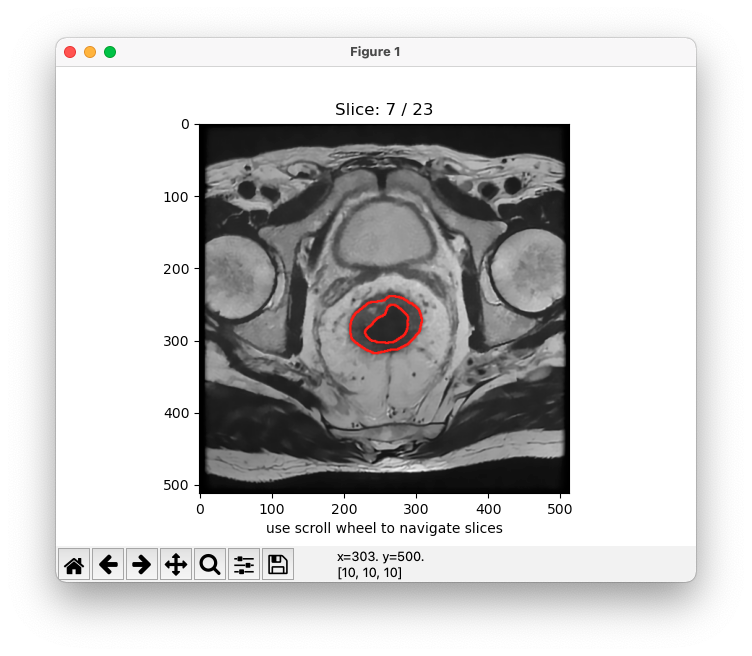
\includegraphics[width=0.9\textwidth]{../images/example_redcont.png}

    \caption{Identified tumor area inside the red contours.}
    \label{quickstart}
    
\end{figure}

\clearpage
\newpage

\subsubsection{mask}


The output is the stack of predicted binary [0, 1] mask of input each slice.
To get it:

\begin{lstlisting}[language = bash]
python -m MRIsegm --dir='/path/to/input/series/'  --mask
\end{lstlisting}

\begin{figure}[ht]

    \centering
    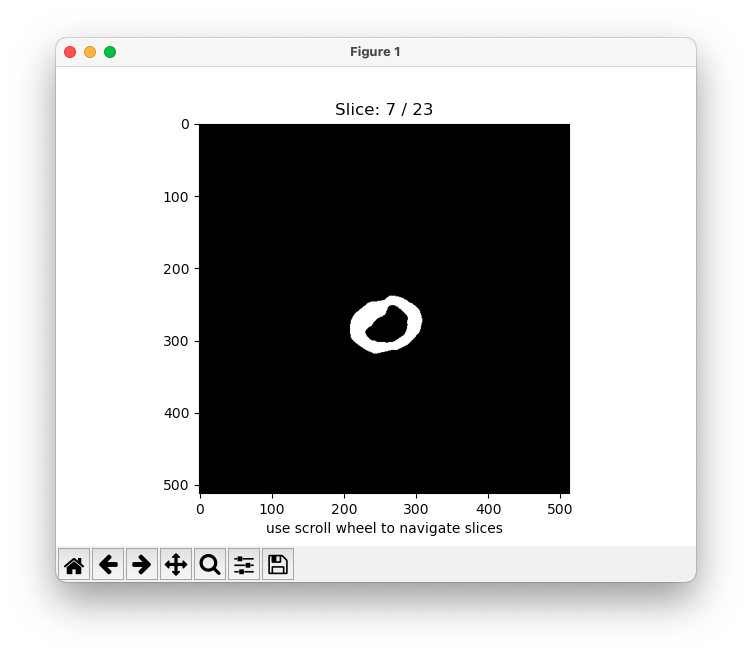
\includegraphics[width=0.9\textwidth]{../images/example_mask.png}

    \caption{Binary mask of the segmented tumor area.}
    \label{mask}
    
\end{figure}

\clearpage
\newpage

\subsubsection{density}

The output is the stack of probability map between 0. and 1. of each input slice over the original image.
To get it:

\begin{lstlisting}[language = bash]
python -m MRIsegm --dir='/path/to/input/series/'  --density
\end{lstlisting}

\begin{figure}[ht]

    \centering
    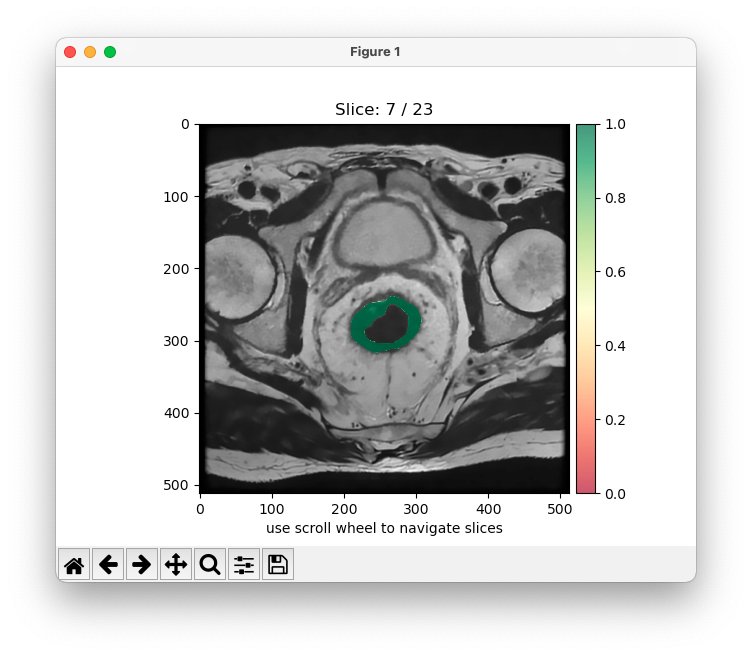
\includegraphics[width=0.9\textwidth]{../images/example_density.png}

    \caption{Probability map of the segmented tumor area.}
    \label{density}
    
\end{figure}

\clearpage
\newpage

\subsubsection{3D}

The output is a 3D mesh plot of the segmented areas.
To get it:

\begin{lstlisting}[language = bash]
python -m MRIsegm --dir='/path/to/input/series/'  --3D
\end{lstlisting}

\begin{figure}[ht]

    \centering
    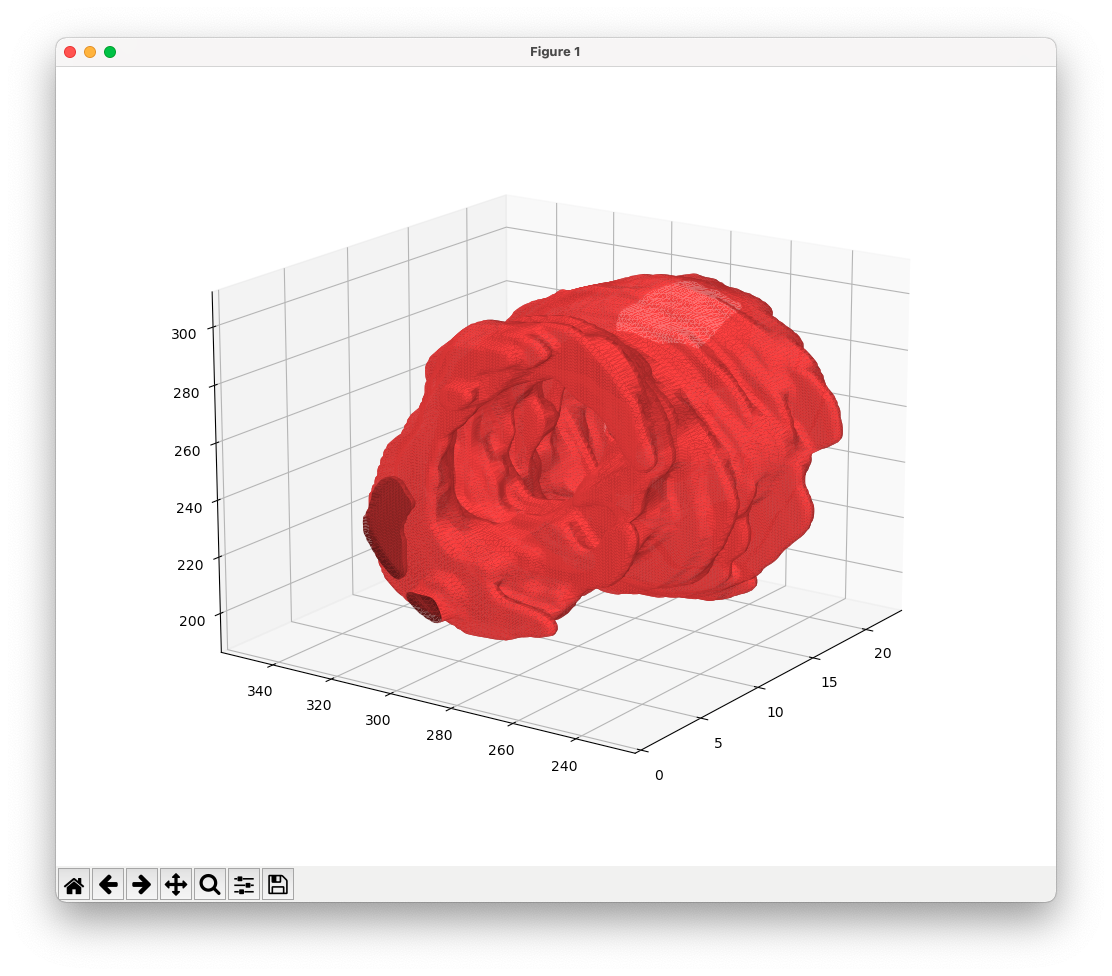
\includegraphics[width=0.9\textwidth]{../images/example_3D.png}

    \caption{3D mesh of the segmented areas.}
    \label{3D}
    
\end{figure}

\end{document}